\section{自动化工具}%hbk

\subsection{页面格式}
    \begin{frame}
        \frametitle{页码格式修改的需要}
        \begin{itemize}
            \item 扉页,或目录,不应该有页码,或者应该单独计页码数
            \item 页码位置有要求(页面底部正中间,右下角,右上角)
        \end{itemize}
    \end{frame}
    
    \begin{frame}
        \frametitle{page计数器}
        \begin{itemize}
            \item 页码有个专门的page计数器,每隔一页,计数器加一,然后按照你设置的格式要求,选择是否打印页码,打印在何处,页码字体等等 \pause
            \item 使用$\backslash$pagenumbering命令对计数器内的值进行调整
                \begin{itemize}
                    \item gobble:没有页码
                    \item arabic:阿拉伯数字
                    \item roman:罗马数字
                \end{itemize}
            \item 打开prac里面的page.tex试试
        \end{itemize}
    \end{frame}

    \begin{frame}
        \frametitle{其他设置}
        \begin{itemize}
            \item 页面尺寸
            \item 分栏
            \item ......
        \end{itemize}
        一般模板会帮你设置好,有需要再上网查,或者看手册
    \end{frame}


\subsection{目录}
    \begin{frame}
        \frametitle{生成目录}
        \begin{itemize}
            \item tableofcontents
            \item 需要编译两次
            \item listoffigures和listoftables命令
            \item 练习catalog
        \end{itemize}
    \end{frame}

    \begin{frame}
        \frametitle{目录内容、格式}
        \begin{itemize}
            \item 读入目录文件
            \item 目录、编号的深度和格式
            \item tocbibind, tocloft, titletoc, minitoc等宏包的使用(手添目录,修改间距,修改字体,一二三级子目录标题等等)
        \end{itemize}
        需要的时候网上查,或者看手册
    \end{frame}



\subsection{交叉引用}
    \begin{frame}
        \frametitle{交叉引用的需求}
        \begin{verse}
        现在是8102年,我正在使用\LaTeX 写我的黎曼猜想证明……\\
        好,这一步可以从引理8推出来,让我康康它在哪一页。\\
        (刷刷刷,鼠标往前滚……\\
        卧槽,我怎么找不到我的引理8了。\\
        (哦,它在第17页,写上……\\
        前面好像不太缜密,我再补补。\\
        太好了,这一步也可以从引理8推出来,让我康康它在哪一页。\\
        卧槽,怎么17页没有引理8,\text{($\bigodot$o$\bigodot$)?}\\
        哦,跑到19页了……不对,我前面那里也要改\text{|($\circledS$\_\_$\circledS$)|}
        \end{verse}
    \end{frame}
    
    \begin{frame}[fragile]
        \frametitle{简单使用}
        只需要两步:
\begin{lstlisting}
% 定义标签
\label{•}

% 引用标签,ref编号引用,pageref页码引用
\ref{•}
\pageref{•} 
\end{lstlisting}
        打开练习CrossReferences
    \end{frame}
    
    \begin{frame}[fragile]
        \frametitle{标签的命名规范}
        \begin{itemize}
            \item 在做练习的过程中,请注意文本中对图片狮子和公式的命名方式:\verb|fig:lion|, \verb|eq:1|
            \item 命名规范非常重要,方便记忆,方便查找,方便分类。
        \end{itemize}
        \begin{figure}
        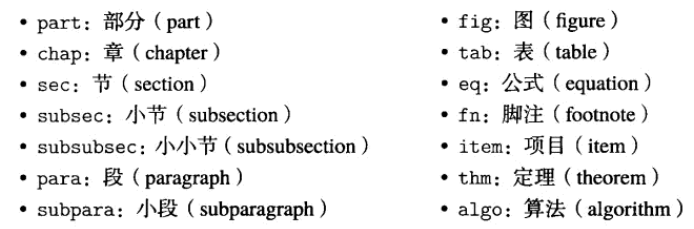
\includegraphics[width=\textwidth]{img//HowToName.png}
        \end{figure}
    \end{frame}
    
    \begin{frame}[fragile]
        \frametitle{pdf文件功能上的拓展}
        pdf文档支持很多特殊功能,如文档标签,超链接,电子表单等等,\LaTeX 也可以输出这样的功能,比如超链接,而这只需要添加一个宏包。
\begin{lstlisting}
% 在导言区(你最好不要忘了导言区是哪里)
% 插入下面的宏包
\usepackage{hyperref}
% 插入后,交叉引用会自动变为超链接。同样,至少编译两次
\end{lstlisting}
        \begin{itemize}
            \item 为刚才做的CrossReferences添加hyperref宏包,增加超链接
            \item 进入练习Hyperref中,猜测理解hypersetup中的内容。在pdf文件中,依次点击目录,公式标签,网页超链接,文件超链接,以及语句的链接。语句的链接可以注意一下,看看它是用了怎样的命令定位的。
        \end{itemize}
    \end{frame}



\subsection{索引}

    \begin{frame}[fragile]
    其实我觉得很多同学不知道什么叫索引。(快来打脸)
    \begin{figure}
    \centering
    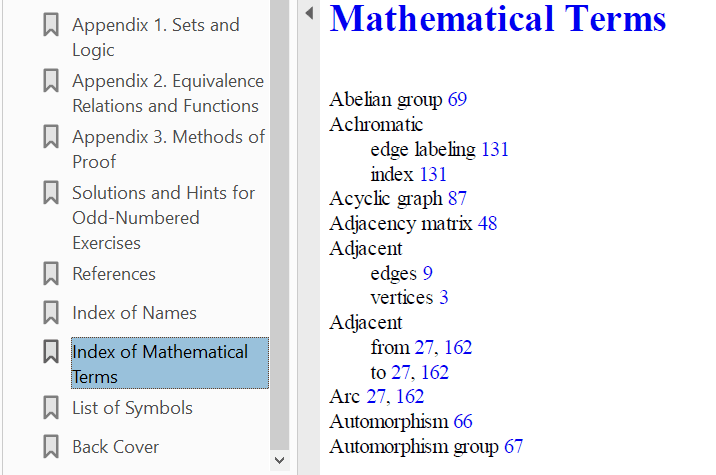
\includegraphics[width = 0.7\textwidth]{img//index.png}
    \end{figure}
    \end{frame}

    \begin{frame}[fragile]
    \frametitle{步骤}
    对tex文件,你需要做:
\begin{lstlisting}
导言区使用\makeindex
导言区调用makeidx宏包
需要索引的地方,使用\index{•}标记
在放索引的地方(通常是末尾),使用\printindex命令
\end{lstlisting}
    编译时,你需要:
\begin{lstlisting}
xelatex file_name
makeindex file_name
xelatex file_name
\end{lstlisting}
    注意:
    \begin{itemize}
        \item 配置好你的makeindex
        \item 不要忘了编译的次数和顺序
    \end{itemize}
    进入练习WordIndex,看看能不能编译出两个tex文件的索引
    \end{frame}

\subsection{文献引用}

    \begin{frame}[fragile]
        这块不细讲了,主要是编译的顺序
\begin{lstlisting}
xelatex filename
bibtex filename
xelatex filename
xelatex filename
\end{lstlisting}
         \begin{itemize}
             \item 在练习bib中按照上面的编译顺序,看看能否生成样例中的文件
             \item 在tex文件中用的指令,可去网上具体了解。
             \item 引用可以在tex文件中自己写,但用的比较多的是写在bib文件中(有专门的管理软件),最后导入,生成引用
         \end{itemize}
    \end{frame}



